\documentclass[fontset=windows]{article}
\usepackage[margin=1in]{geometry}
\usepackage{ctex}
\usepackage{setspace}
\usepackage{lipsum}
\usepackage{graphicx}
\usepackage{caption}
\usepackage{subcaption}
\usepackage[colorlinks=true,linkcolor=red]{hyperref}

\graphicspath{{figures/}}

\title{\heiti\zihao{2} Common-Source Stage with Degeneration}
\author{\songti zrrraa}
\date{2023.11.22}

\begin{document}
\maketitle
\thispagestyle{empty}

\section*{Degenerated CS Stage}

We assume the $\lambda=0$. 

\subsection*{Step \uppercase\expandafter{\romannumeral1}: Bias Conditions}

\begin{figure}[htbp]
    \centering
    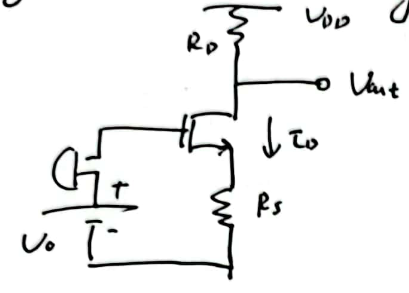
\includegraphics[scale=0.8]{1.jpg}
    \captionsetup{labelformat=empty}
    \caption{}
    \label{1}
\end{figure}

$$V_D=V_GS+I_DR_S$$

For saturation zone, $V_{DS}\geq V_{GS}-V_{TH}$. 

$$I_D=\frac{1}{2}\mu_nC_{ox}\frac{W}{L}(V_{GS}-V_{TH})^2$$

Drain voltage=$V_{DD}-I_DR_D$

\subsection*{Step \uppercase\expandafter{\romannumeral2}: Gain, I/O Impedances}

\begin{figure}[htbp]
    \centering
    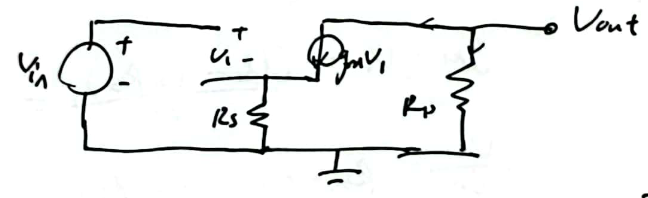
\includegraphics[scale=0.8]{2.jpg}
    \captionsetup{labelformat=empty}
    \caption{}
    \label{2}
\end{figure}

$$g_mv_1=-\frac{v_{out}}{R_D}$$

$$v_{in}=V_1+g_mv_1*R_S$$

$$\Longrightarrow\frac{v_{out}}{v_{in}}=-\frac{R_D}{\frac{1}{g_m}+R_s}$$

Therefore: 

$$A_v=-\frac{Resistance \ tied \ between \ Drain \ and \ AC \ Ground}{\frac{1}{g_m}+Resistance \ tied \ between \ Source \ and \ AC \ Ground}$$

\subsection*{Example}

\begin{figure}[htbp]
    \centering
    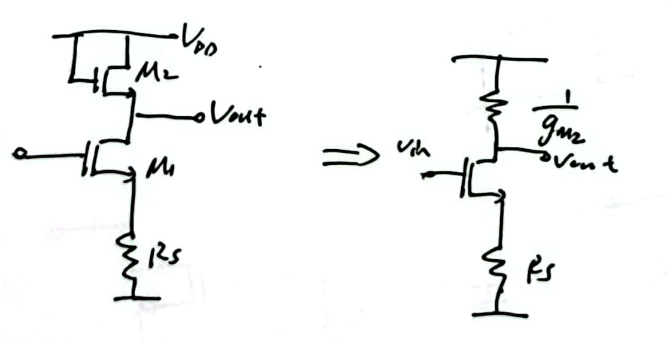
\includegraphics[scale=0.8]{3.jpg}
    \captionsetup{labelformat=empty}
    \caption{}
    \label{3}
\end{figure}

$$A_v=-\frac{\frac{1}{g_{m2}}}{\frac{1}{g_{m1}}+R_S}$$

So why is gain less with degenerated CS stage? 

\begin{figure}[htbp]
    \centering
    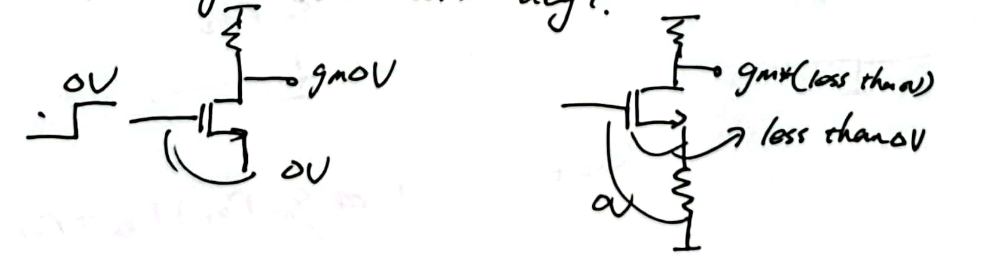
\includegraphics[scale=0.8]{4.jpg}
    \captionsetup{labelformat=empty}
    \caption{}
    \label{4}
\end{figure}

From the picture we can easily see the change of voltage between Gate and Source is less with deg. 
So the gain is less. 

\section*{Let's build a current source}

\begin{figure}[htbp]
    \centering
    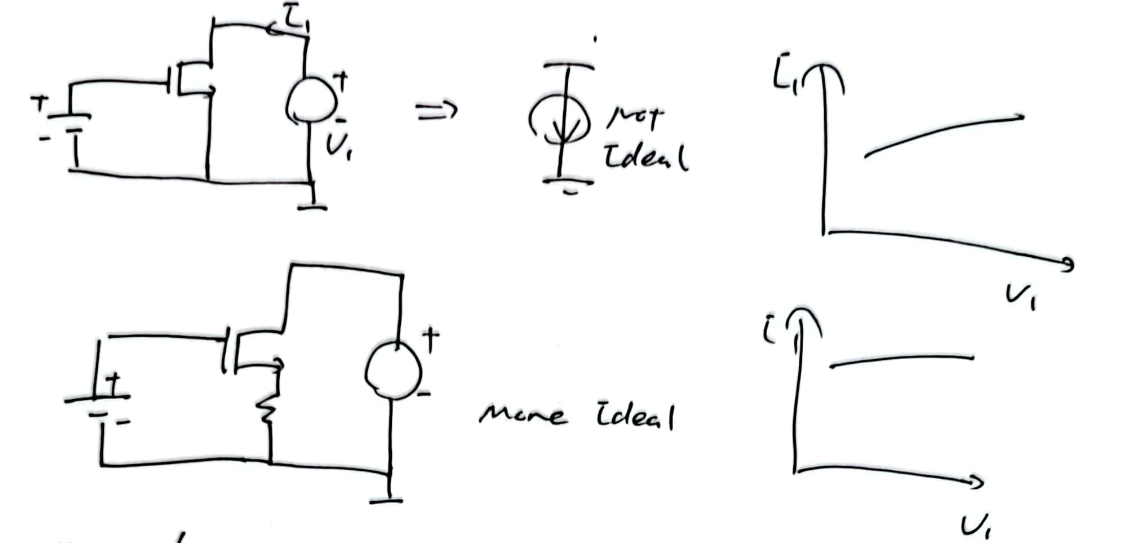
\includegraphics[scale=0.6]{5.jpg}
    \captionsetup{labelformat=empty}
    \caption{}
    \label{5}
\end{figure}

We draw the I/V relationship between Drain and Source, it's clear that the CS stage with degeneration is more smooth. 
Or we can call it more ideal, as a current source. That's the meaning of degeneration. 

\subsection*{Small-Signal Imp}

\begin{figure}[htbp]
    \centering
    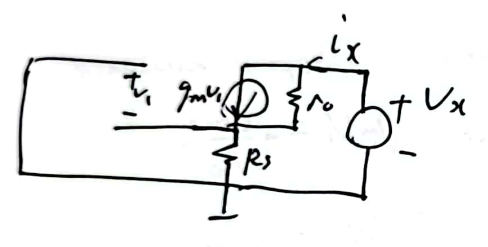
\includegraphics[scale=0.8]{6.jpg}
    \captionsetup{labelformat=empty}
    \caption{}
    \label{6}
\end{figure}

Calculate the output impedance. 

$$i_xR_S=-v_1$$

$$g_mv_1+\frac{v_x-i_xR_S}{r_o}=i_x$$

$$\Longrightarrow \frac{v_x}{i_x}=R_S+r_o+g_mR_Sr_o=(1+g_mr_o)R_S+r_o$$

\subsection*{Example}

\begin{figure}[htbp]
    \centering
    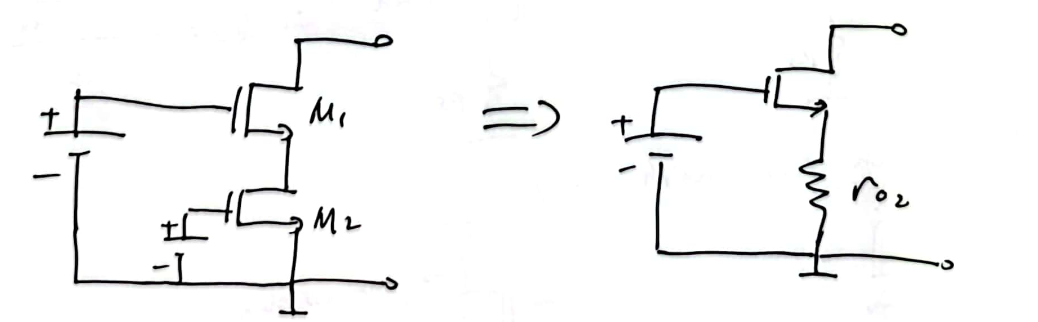
\includegraphics[scale=0.8]{7.jpg}
    \captionsetup{labelformat=empty}
    \caption{}
    \label{7}
\end{figure}

$$R_{out}=(1+g_mr_{o1})r_{o2}+r_{o1}$$

This structure has a special name: Cascode. We will learn it after. 

\section*{Link}

\href{https://www.bilibili.com/video/BV1FD4y1R7Ah?p=38&vd_source=1d0c07486a3bd3b0adb8ac548bf6453e}{Razavi Electronics Circuits 1: lectrue 38}
\end{document}